%% Condensed from dissertacao-en/chapters/cap6-framework.tex @295dde3.
\chapter{The Decision Framework, Evaluated}
\label{chap:framework}

If accuracy near-ties and costs decide, how should a practitioner
choose? This chapter submits the decision framework to evaluation by
three studies on the benchmark's own datasets (18; 17 where the FM
family participates): a negative result on learned routing, a
positive result on a fixed-policy reading, and a registered
weighted-regret analysis that locates when the recommendation
flips. Full tables and the multi-criteria star matrix are in the
extended report.

\section{Regret and the LODO protocol}
\label{sec:cap6-regret}

Normalized regret measures, per dataset, how far a choice sits from
that dataset's best model on the primary metric, scaled to $[0,1]$
(on \texttt{adult}, picking the best GBDT costs regret 0.10; the
best deep model, 0.60). Policies are evaluated under
leave-one-dataset-out (LODO) where learning is involved: the router
is trained on 17 datasets and judged on the held-out one --- the
most rigorous protocol available at $N{=}18$.

\section{A negative and a positive result}
\label{sec:cap6-router}

\textbf{Routing by meta-features does not generalize.} A
decision-tree router over dataset meta-features hits the correct
model family on 0.11 of held-out datasets against 0.44 for the
trivial rule ``always predict the most frequent family'' with 11
models, and 0.72 against 0.78 with 14 (including the 2026
generation); a registered robustness sweep over eight router
configurations leaves the conclusion unchanged in every cell. The
most likely cause is structural: each LODO round trains on 17
examples, a sample where any partition by meta-features is dominated
by the noise of individual reversals.

\textbf{A fixed policy is regret-optimal.}
Table~\ref{tab:regret-lodo} evaluates fixed policies descriptively
(only the tree is a learned object under LODO; ``Always-FM'' is the
within-family oracle --- the family's ceiling). At 14 models the
oracle has median regret 0.000 and mean 0.021; the \emph{executable}
always-TabFM also has median 0.000 with mean 0.080, pulled by a
single worst case of 1.000 on
\texttt{telco\_\allowbreak customer\_\allowbreak churn} --- the
dataset whose declared preprocessing idiosyncrasy penalizes the FM
(Chapter~\ref{chap:metodologia}); always-TabPFN sits at median 0.242.
By the mean, the LODO tree (0.051) beats every executable fixed
policy --- the headline ``FM first'' is a median statement about a
family ceiling, and the chapter says so wherever it is used.

\begin{table}[htb]
\centering
\caption[Normalized regret of policies under LODO]{Mean and median
normalized regret of the LODO tree and fixed policies, at 11 and at
14 models. ``Always-FM'' is the within-family oracle; the executable
policies are listed separately.}
\label{tab:regret-lodo}
\small
\begin{tabular}{lcccc}
\toprule
Policy & mean @11 & median @11 & mean @14 & median @14 \\
\midrule
Tree (LODO)        & 0.228 & 0.145 & 0.051 & 0.000 \\
Always-GBDT        & 0.249 & 0.168 & 0.305 & 0.291 \\
Always-DL          & 0.189 & 0.132 & 0.313 & 0.349 \\
\textbf{Always-FM} & \textbf{0.115} & \textbf{0.018} & \textbf{0.021} &
\textbf{0.000} \\
\midrule
Always-TabFM (executable)  & --- & --- & 0.080 & 0.000 \\
Always-TabPFN (executable) & 0.115 & 0.018 & 0.261 & 0.242 \\
\bottomrule
\end{tabular}
\end{table}

\section{When the recommendation flips: weighted regret (E2)}
\label{sec:regret-ponderado}
\label{sec:e2-resultados}

E2 is a \emph{registered analysis} (design fixed before execution;
not a pre-registration, since the accuracy-only endpoint was already
known): the per-dataset score becomes
$S = w \cdot r_{\mathrm{acc}} + (1-w) \cdot r_{\mathrm{lat}}$, with
rank-normalized accuracy and latency, swept over $w$
(Figure~\ref{fig:cap6-regret}). ``FM first'' is regret-optimal by
the median only while $w \geq 0.9$: shifting \textbf{10--20\%} of
the weight from accuracy to latency hands the lead to the cheaper
families (by the mean, 20--30\%). The band is a property of the
design's rank normalization: min--max alternatives move the flip to
20--25\% (logarithmic) and 30--35\% (linear) --- the direction is
the same, and the rank normalization flips earliest. The latency
proxy was also stress-tested: re-running the sweep with latency
measured on a small and a large dataset leaves the crossover
identical, with the always-GBDT zone shifting $\pm0.1$ --- in the
direction opposite to the one anticipated in the record.

\begin{figure}[htb]
\centering
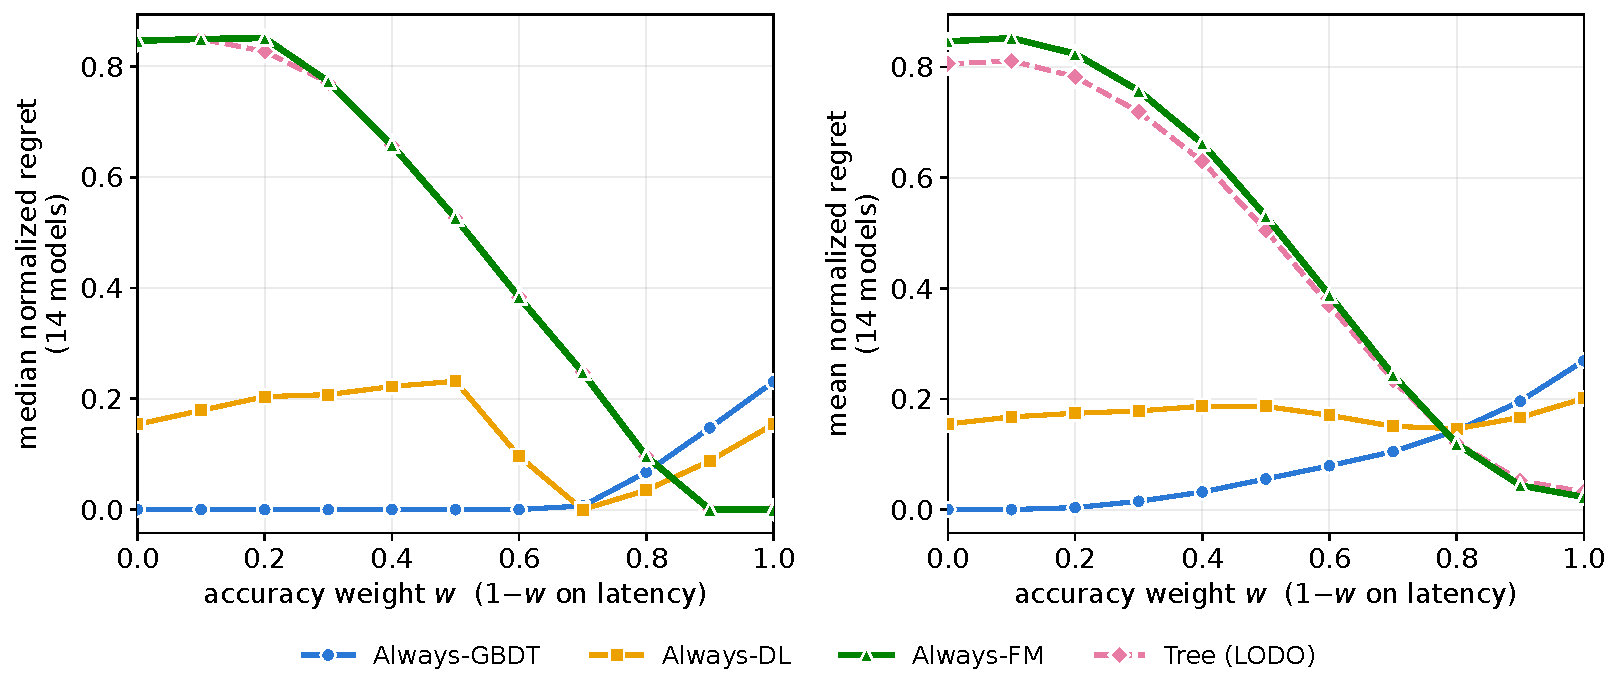
\includegraphics[width=\linewidth]{images/lodo_weighted_regret.pdf}
\caption[Weighted regret against the latency weight]{Median (left)
and mean (right) normalized regret of the policies as the weight
moves from accuracy ($w{=}1$) to latency.}
\label{fig:cap6-regret}
\end{figure}

\section{The resulting framework: decision by constraints}
\label{sec:arcabouco-resultante}

The three studies justify a constraint-first flowchart
(Figure~\ref{fig:cap6-flow}): latency budget, architectural limits
(>10 classes; context caps), and the requirement of auditable
explanations --- GBDTs are accepted in regulated practice via
attribution-based explanations, which is an acceptance criterion,
not strict intrinsic interpretability --- are checked in order;
with no active constraint, foundation model first (TabPFN mature;
TabFM frontier, v1.0.1 caveats). The flowchart is a \emph{synthesis
of the three studies, not an evaluated policy}: no end-to-end
accuracy claim is attached to following it.

\begin{figure}[htb]
\centering
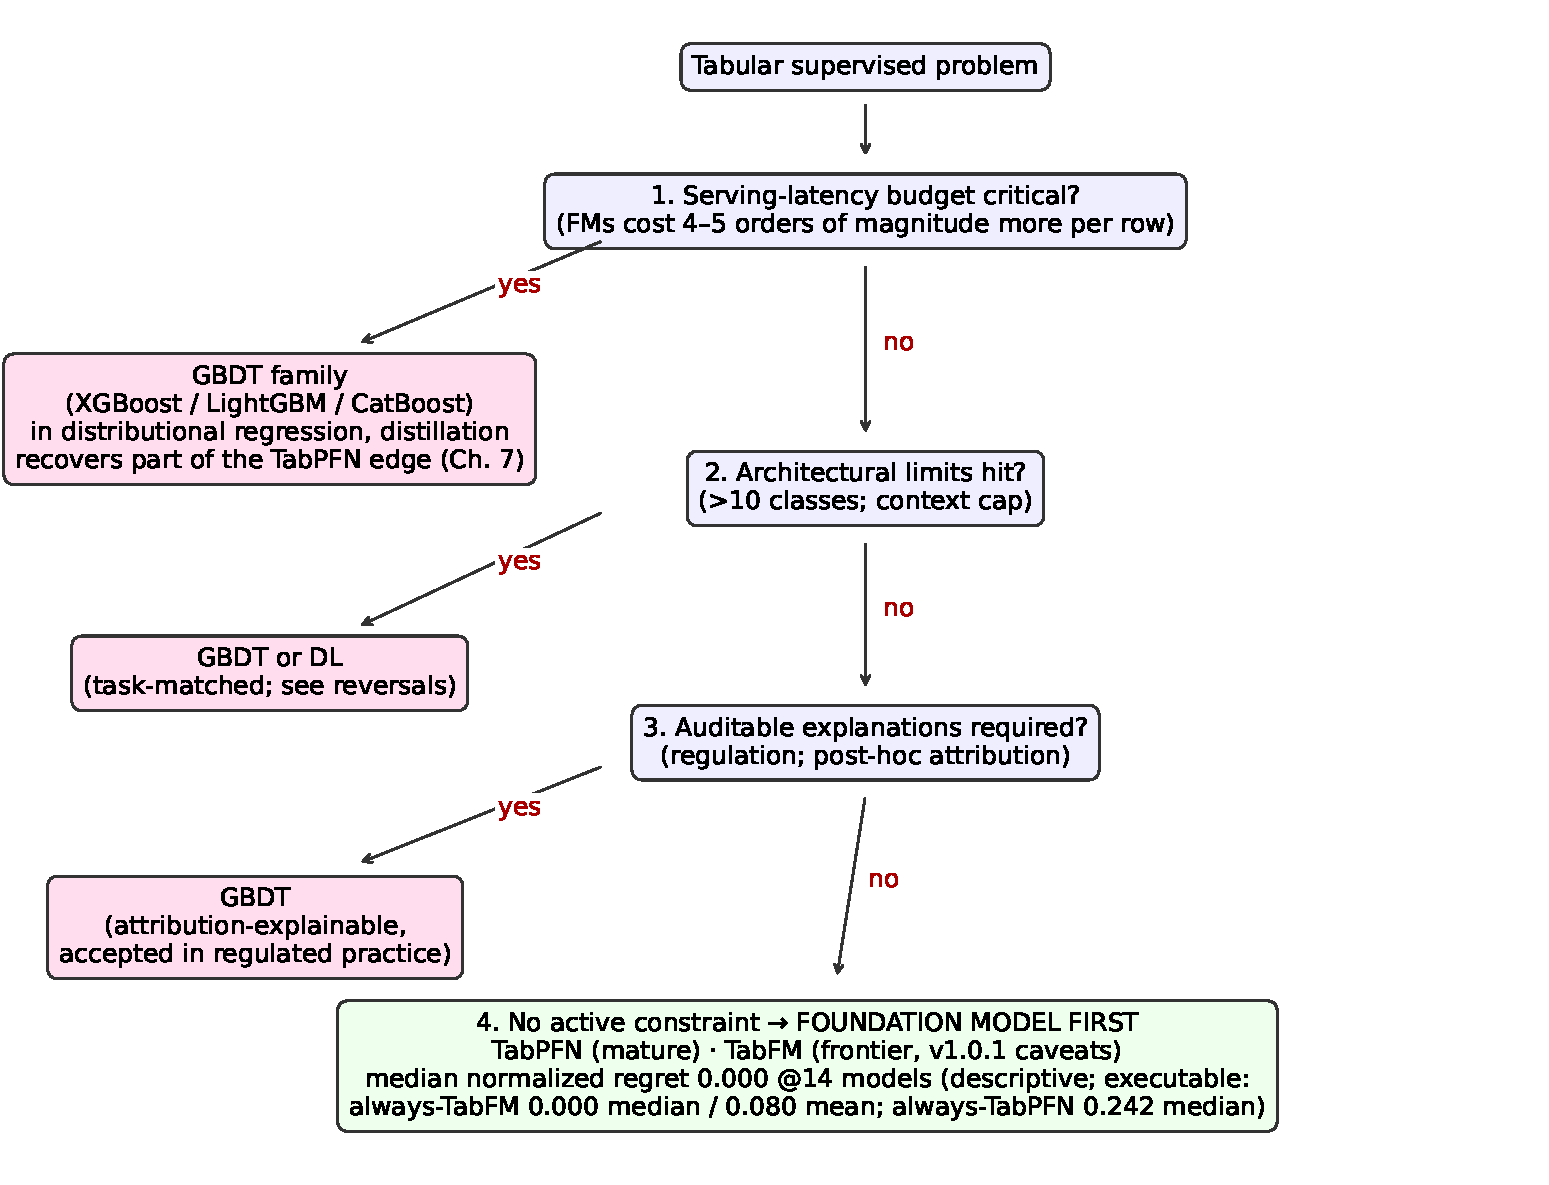
\includegraphics[width=0.9\linewidth]{images/decision_flowchart_14_en.pdf}
\caption[The evaluated decision flowchart]{The four-constraint
flowchart at 14 models. Each box is a constraint verifiable a
priori.}
\label{fig:cap6-flow}
\end{figure}

\emph{Limitations, briefly: regret compares models within this
benchmark's grid; the flip band depends on the score normalization
(10--20\% by ranks; up to 35\% under min--max variants); latency
enters by a single-machine proxy; only the tree was evaluated under
LODO; and the flowchart inherits every caveat of
Chapter~\ref{chap:benchmark}'s measurements.}
